\documentclass[1p]{elsarticle_modified}
%\bibliographystyle{elsarticle-num}

%\usepackage[colorlinks]{hyperref}
%\usepackage{abbrmath_seonhwa} %\Abb, \Ascr, \Acal ,\Abf, \Afrak
\usepackage{amsfonts}
\usepackage{amssymb}
\usepackage{amsmath}
\usepackage{amsthm}
\usepackage{scalefnt}
\usepackage{amsbsy}
\usepackage{kotex}
\usepackage{caption}
\usepackage{subfig}
\usepackage{color}
\usepackage{graphicx}
\usepackage{xcolor} %% white, black, red, green, blue, cyan, magenta, yellow
\usepackage{float}
\usepackage{setspace}
\usepackage{hyperref}

\usepackage{tikz}
\usetikzlibrary{arrows}

\usepackage{multirow}
\usepackage{array} % fixed length table
\usepackage{hhline}

%%%%%%%%%%%%%%%%%%%%%
\makeatletter
\renewcommand*\env@matrix[1][\arraystretch]{%
	\edef\arraystretch{#1}%
	\hskip -\arraycolsep
	\let\@ifnextchar\new@ifnextchar
	\array{*\c@MaxMatrixCols c}}
\makeatother %https://tex.stackexchange.com/questions/14071/how-can-i-increase-the-line-spacing-in-a-matrix
%%%%%%%%%%%%%%%

\usepackage[normalem]{ulem}

\newcommand{\msout}[1]{\ifmmode\text{\sout{\ensuremath{#1}}}\else\sout{#1}\fi}
%SOURCE: \msout is \stkout macro in https://tex.stackexchange.com/questions/20609/strikeout-in-math-mode

\newcommand{\cancel}[1]{
	\ifmmode
	{\color{red}\msout{#1}}
	\else
	{\color{red}\sout{#1}}
	\fi
}

\newcommand{\add}[1]{
	{\color{blue}\uwave{#1}}
}

\newcommand{\replace}[2]{
	\ifmmode
	{\color{red}\msout{#1}}{\color{blue}\uwave{#2}}
	\else
	{\color{red}\sout{#1}}{\color{blue}\uwave{#2}}
	\fi
}

\newcommand{\Sol}{\mathcal{S}} %segment
\newcommand{\D}{D} %diagram
\newcommand{\A}{\mathcal{A}} %arc


%%%%%%%%%%%%%%%%%%%%%%%%%%%%%5 test

\def\sl{\operatorname{\textup{SL}}(2,\Cbb)}
\def\psl{\operatorname{\textup{PSL}}(2,\Cbb)}
\def\quan{\mkern 1mu \triangleright \mkern 1mu}

\theoremstyle{definition}
\newtheorem{thm}{Theorem}[section]
\newtheorem{prop}[thm]{Proposition}
\newtheorem{lem}[thm]{Lemma}
\newtheorem{ques}[thm]{Question}
\newtheorem{cor}[thm]{Corollary}
\newtheorem{defn}[thm]{Definition}
\newtheorem{exam}[thm]{Example}
\newtheorem{rmk}[thm]{Remark}
\newtheorem{alg}[thm]{Algorithm}

\newcommand{\I}{\sqrt{-1}}
\begin{document}

%\begin{frontmatter}
%
%\title{Boundary parabolic representations of knots up to 8 crossings}
%
%%% Group authors per affiliation:
%\author{Yunhi Cho} 
%\address{Department of Mathematics, University of Seoul, Seoul, Korea}
%\ead{yhcho@uos.ac.kr}
%
%
%\author{Seonhwa Kim} %\fnref{s_kim}}
%\address{Center for Geometry and Physics, Institute for Basic Science, Pohang, 37673, Korea}
%\ead{ryeona17@ibs.re.kr}
%
%\author{Hyuk Kim}
%\address{Department of Mathematical Sciences, Seoul National University, Seoul 08826, Korea}
%\ead{hyukkim@snu.ac.kr}
%
%\author{Seokbeom Yoon}
%\address{Department of Mathematical Sciences, Seoul National University, Seoul, 08826,  Korea}
%\ead{sbyoon15@snu.ac.kr}
%
%\begin{abstract}
%We find all boundary parabolic representation of knots up to 8 crossings.
%
%\end{abstract}
%\begin{keyword}
%    \MSC[2010] 57M25 
%\end{keyword}
%
%\end{frontmatter}

%\linenumbers
%\tableofcontents
%
\newcommand\colored[1]{\textcolor{white}{\rule[-0.35ex]{0.8em}{1.4ex}}\kern-0.8em\color{red} #1}%
%\newcommand\colored[1]{\textcolor{white}{ #1}\kern-2.17ex	\textcolor{white}{ #1}\kern-1.81ex	\textcolor{white}{ #1}\kern-2.15ex\color{red}#1	}

{\Large $\underline{12n_{0866}~(K12n_{0866})}$}

\setlength{\tabcolsep}{10pt}
\renewcommand{\arraystretch}{1.6}
\vspace{1cm}\begin{tabular}{m{100pt}>{\centering\arraybackslash}m{274pt}}
\multirow{5}{120pt}{
	\centering
	\includegraphics[width=112pt]{../../../GIT/diagram.site/Diagrams/png/2955_12n_0866.png}\\
\ \ \ A knot diagram\footnotemark}&
\allowdisplaybreaks
\textbf{Linearized knot diagam} \\
\cline{2-2}
 &
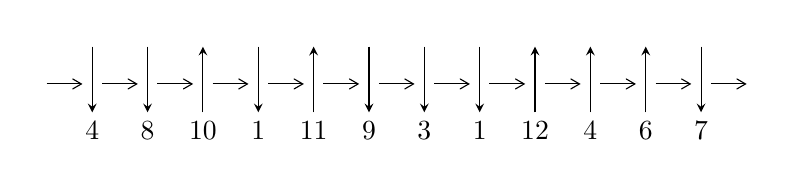
\begin{tikzpicture}[x=20pt, y=17pt]
	% nodes
	\node (C0) at (0, 0) {};
	\node (C1) at (1, 0) {};
	\node (C1U) at (1, +1) {};
	\node (C1D) at (1, -1) {4};

	\node (C2) at (2, 0) {};
	\node (C2U) at (2, +1) {};
	\node (C2D) at (2, -1) {8};

	\node (C3) at (3, 0) {};
	\node (C3U) at (3, +1) {};
	\node (C3D) at (3, -1) {10};

	\node (C4) at (4, 0) {};
	\node (C4U) at (4, +1) {};
	\node (C4D) at (4, -1) {1};

	\node (C5) at (5, 0) {};
	\node (C5U) at (5, +1) {};
	\node (C5D) at (5, -1) {11};

	\node (C6) at (6, 0) {};
	\node (C6U) at (6, +1) {};
	\node (C6D) at (6, -1) {9};

	\node (C7) at (7, 0) {};
	\node (C7U) at (7, +1) {};
	\node (C7D) at (7, -1) {3};

	\node (C8) at (8, 0) {};
	\node (C8U) at (8, +1) {};
	\node (C8D) at (8, -1) {1};

	\node (C9) at (9, 0) {};
	\node (C9U) at (9, +1) {};
	\node (C9D) at (9, -1) {12};

	\node (C10) at (10, 0) {};
	\node (C10U) at (10, +1) {};
	\node (C10D) at (10, -1) {4};

	\node (C11) at (11, 0) {};
	\node (C11U) at (11, +1) {};
	\node (C11D) at (11, -1) {6};

	\node (C12) at (12, 0) {};
	\node (C12U) at (12, +1) {};
	\node (C12D) at (12, -1) {7};
	\node (C13) at (13, 0) {};

	% arrows
	\draw[->,>={angle 60}]
	(C0) edge (C1) (C1) edge (C2) (C2) edge (C3) (C3) edge (C4) (C4) edge (C5) (C5) edge (C6) (C6) edge (C7) (C7) edge (C8) (C8) edge (C9) (C9) edge (C10) (C10) edge (C11) (C11) edge (C12) (C12) edge (C13) ;	\draw[->,>=stealth]
	(C1U) edge (C1D) (C2U) edge (C2D) (C3D) edge (C3U) (C4U) edge (C4D) (C5D) edge (C5U) (C6U) edge (C6D) (C7U) edge (C7D) (C8U) edge (C8D) (C9D) edge (C9U) (C10D) edge (C10U) (C11D) edge (C11U) (C12U) edge (C12D) ;
	\end{tikzpicture} \\
\hhline{~~} \\& 
\textbf{Solving Sequence} \\ \cline{2-2} 
 &
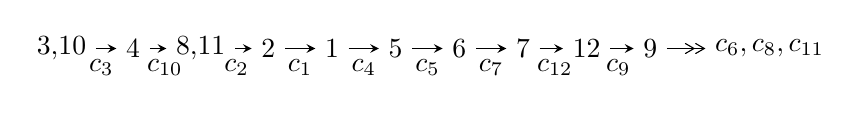
\begin{tikzpicture}[x=23pt, y=7pt]
	% node
	\node (A0) at (-1/8, 0) {3,10};
	\node (A1) at (1, 0) {4};
	\node (A2) at (33/16, 0) {8,11};
	\node (A3) at (25/8, 0) {2};
	\node (A4) at (33/8, 0) {1};
	\node (A5) at (41/8, 0) {5};
	\node (A6) at (49/8, 0) {6};
	\node (A7) at (57/8, 0) {7};
	\node (A8) at (65/8, 0) {12};
	\node (A9) at (73/8, 0) {9};
	\node (C1) at (1/2, -1) {$c_{3}$};
	\node (C2) at (3/2, -1) {$c_{10}$};
	\node (C3) at (21/8, -1) {$c_{2}$};
	\node (C4) at (29/8, -1) {$c_{1}$};
	\node (C5) at (37/8, -1) {$c_{4}$};
	\node (C6) at (45/8, -1) {$c_{5}$};
	\node (C7) at (53/8, -1) {$c_{7}$};
	\node (C8) at (61/8, -1) {$c_{12}$};
	\node (C9) at (69/8, -1) {$c_{9}$};
	\node (A10) at (11, 0) {$c_{6},c_{8},c_{11}$};

	% edge
	\draw[->,>=stealth]	
	(A0) edge (A1) (A1) edge (A2) (A2) edge (A3) (A3) edge (A4) (A4) edge (A5) (A5) edge (A6) (A6) edge (A7) (A7) edge (A8) (A8) edge (A9) ;
	\draw[->>,>={angle 60}]	
	(A9) edge (A10);
\end{tikzpicture} \\ 

\end{tabular} \\

\footnotetext{
The image of knot diagram is generated by the software ``\textbf{Draw programme}" developed by Andrew Bartholomew(\url{http://www.layer8.co.uk/maths/draw/index.htm\#Running-draw}), where we modified some parts for our purpose(\url{https://github.com/CATsTAILs/LinksPainter}).
}\phantom \\ \newline 
\centering \textbf{Ideals for irreducible components\footnotemark of $X_{\text{par}}$} 
 
\begin{align*}
I^u_{1}&=\langle 
1.24188\times10^{496} u^{100}-3.45972\times10^{496} u^{99}+\cdots+4.38110\times10^{498} b-8.43502\times10^{499},\\
\phantom{I^u_{1}}&\phantom{= \langle  }-6.68237\times10^{501} u^{100}+1.69590\times10^{502} u^{99}+\cdots+7.40551\times10^{503} a+3.34460\times10^{505},\\
\phantom{I^u_{1}}&\phantom{= \langle  }u^{101}-2 u^{100}+\cdots-18346 u-3931\rangle \\
I^u_{2}&=\langle 
-3.33238\times10^{33} u^{30}+1.40429\times10^{33} u^{29}+\cdots+3.70136\times10^{33} b+8.89806\times10^{33},\\
\phantom{I^u_{2}}&\phantom{= \langle  }2.33080\times10^{34} u^{30}+6.01457\times10^{33} u^{29}+\cdots+1.85068\times10^{34} a+5.60898\times10^{34},\;u^{31}- u^{30}+\cdots+3 u+1\rangle \\
\\
\end{align*}
\raggedright * 2 irreducible components of $\dim_{\mathbb{C}}=0$, with total 132 representations.\\
\footnotetext{All coefficients of polynomials are rational numbers. But the coefficients are sometimes approximated in decimal forms when there is not enough margin.}
\newpage
\renewcommand{\arraystretch}{1}
\centering \section*{I. $I^u_{1}= \langle 1.24\times10^{496} u^{100}-3.46\times10^{496} u^{99}+\cdots+4.38\times10^{498} b-8.44\times10^{499},\;-6.68\times10^{501} u^{100}+1.70\times10^{502} u^{99}+\cdots+7.41\times10^{503} a+3.34\times10^{505},\;u^{101}-2 u^{100}+\cdots-18346 u-3931 \rangle$}
\flushleft \textbf{(i) Arc colorings}\\
\begin{tabular}{m{7pt} m{180pt} m{7pt} m{180pt} }
\flushright $a_{3}=$&$\begin{pmatrix}1\\0\end{pmatrix}$ \\
\flushright $a_{10}=$&$\begin{pmatrix}0\\u\end{pmatrix}$ \\
\flushright $a_{4}=$&$\begin{pmatrix}1\\- u^2\end{pmatrix}$ \\
\flushright $a_{8}=$&$\begin{pmatrix}0.00902352 u^{100}-0.0229006 u^{99}+\cdots-189.264 u-45.1637\\-0.00283463 u^{100}+0.00789692 u^{99}+\cdots+62.3350 u+19.2532\end{pmatrix}$ \\
\flushright $a_{11}=$&$\begin{pmatrix}u\\- u^3+u\end{pmatrix}$ \\
\flushright $a_{2}=$&$\begin{pmatrix}0.0101284 u^{100}-0.0271243 u^{99}+\cdots-180.804 u-68.4594\\0.00236453 u^{100}-0.00531970 u^{99}+\cdots-89.3719 u-21.0059\end{pmatrix}$ \\
\flushright $a_{1}=$&$\begin{pmatrix}0.0174868 u^{100}-0.0458591 u^{99}+\cdots-356.352 u-116.461\\0.000717401 u^{100}-0.00150781 u^{99}+\cdots-44.5835 u-5.21116\end{pmatrix}$ \\
\flushright $a_{5}=$&$\begin{pmatrix}0.00667899 u^{100}-0.0155294 u^{99}+\cdots-143.768 u-59.2234\\0.00156664 u^{100}-0.00347406 u^{99}+\cdots+7.95421 u-8.67759\end{pmatrix}$ \\
\flushright $a_{6}=$&$\begin{pmatrix}0.00730544 u^{100}-0.0174596 u^{99}+\cdots-149.290 u-57.3470\\0.00189055 u^{100}-0.00468428 u^{99}+\cdots+12.3972 u-4.13842\end{pmatrix}$ \\
\flushright $a_{7}=$&$\begin{pmatrix}0.00618889 u^{100}-0.0150037 u^{99}+\cdots-126.929 u-25.9105\\-0.00283463 u^{100}+0.00789692 u^{99}+\cdots+62.3350 u+19.2532\end{pmatrix}$ \\
\flushright $a_{12}=$&$\begin{pmatrix}0.00373393 u^{100}-0.0102203 u^{99}+\cdots-93.3892 u-35.7880\\0.00459301 u^{100}-0.0114226 u^{99}+\cdots-140.650 u-35.6539\end{pmatrix}$ \\
\flushright $a_{9}=$&$\begin{pmatrix}-0.0138835 u^{100}+0.0364496 u^{99}+\cdots+227.848 u+80.5728\\-0.00415038 u^{100}+0.0118164 u^{99}+\cdots+27.4684 u+6.37850\end{pmatrix}$\\&\end{tabular}
\flushleft \textbf{(ii) Obstruction class $= -1$}\\~\\
\flushleft \textbf{(iii) Cusp Shapes $= 0.00493355 u^{100}-0.0156200 u^{99}+\cdots+258.329 u+60.2116$}\\~\\
\newpage\renewcommand{\arraystretch}{1}
\flushleft \textbf{(iv) u-Polynomials at the component}\newline \\
\begin{tabular}{m{50pt}|m{274pt}}
Crossings & \hspace{64pt}u-Polynomials at each crossing \\
\hline $$\begin{aligned}c_{1},c_{4}\end{aligned}$$&$\begin{aligned}
&u^{101}-7 u^{100}+\cdots-533 u+356
\end{aligned}$\\
\hline $$\begin{aligned}c_{2},c_{7}\end{aligned}$$&$\begin{aligned}
&u^{101}- u^{100}+\cdots+72811 u-14123
\end{aligned}$\\
\hline $$\begin{aligned}c_{3},c_{10}\end{aligned}$$&$\begin{aligned}
&u^{101}-2 u^{100}+\cdots-18346 u-3931
\end{aligned}$\\
\hline $$\begin{aligned}c_{5},c_{11}\end{aligned}$$&$\begin{aligned}
&u^{101}+2 u^{100}+\cdots+641239 u+167761
\end{aligned}$\\
\hline $$\begin{aligned}c_{6}\end{aligned}$$&$\begin{aligned}
&u^{101}-10 u^{100}+\cdots+53 u-7
\end{aligned}$\\
\hline $$\begin{aligned}c_{8}\end{aligned}$$&$\begin{aligned}
&u^{101}-14 u^{99}+\cdots-238884 u+56743
\end{aligned}$\\
\hline $$\begin{aligned}c_{9}\end{aligned}$$&$\begin{aligned}
&u^{101}-12 u^{99}+\cdots+549 u+319
\end{aligned}$\\
\hline $$\begin{aligned}c_{12}\end{aligned}$$&$\begin{aligned}
&u^{101}- u^{100}+\cdots+41 u-2
\end{aligned}$\\
\hline
\end{tabular}\\~\\
\newpage\renewcommand{\arraystretch}{1}
\flushleft \textbf{(v) Riley Polynomials at the component}\newline \\
\begin{tabular}{m{50pt}|m{274pt}}
Crossings & \hspace{64pt}Riley Polynomials at each crossing \\
\hline $$\begin{aligned}c_{1},c_{4}\end{aligned}$$&$\begin{aligned}
&y^{101}-71 y^{100}+\cdots+18234321 y-126736
\end{aligned}$\\
\hline $$\begin{aligned}c_{2},c_{7}\end{aligned}$$&$\begin{aligned}
&y^{101}+51 y^{100}+\cdots-7022994229 y-199459129
\end{aligned}$\\
\hline $$\begin{aligned}c_{3},c_{10}\end{aligned}$$&$\begin{aligned}
&y^{101}-34 y^{100}+\cdots+615503752 y-15452761
\end{aligned}$\\
\hline $$\begin{aligned}c_{5},c_{11}\end{aligned}$$&$\begin{aligned}
&y^{101}-64 y^{100}+\cdots+814720100043 y-28143753121
\end{aligned}$\\
\hline $$\begin{aligned}c_{6}\end{aligned}$$&$\begin{aligned}
&y^{101}-4 y^{100}+\cdots-411 y-49
\end{aligned}$\\
\hline $$\begin{aligned}c_{8}\end{aligned}$$&$\begin{aligned}
&y^{101}-28 y^{100}+\cdots+62222823240 y-3219768049
\end{aligned}$\\
\hline $$\begin{aligned}c_{9}\end{aligned}$$&$\begin{aligned}
&y^{101}-24 y^{100}+\cdots+8075431 y-101761
\end{aligned}$\\
\hline $$\begin{aligned}c_{12}\end{aligned}$$&$\begin{aligned}
&y^{101}-15 y^{100}+\cdots+205 y-4
\end{aligned}$\\
\hline
\end{tabular}\\~\\
\newpage\flushleft \textbf{(vi) Complex Volumes and Cusp Shapes}
$$\begin{array}{c|c|c}  
\text{Solutions to }I^u_{1}& \I (\text{vol} + \sqrt{-1}CS) & \text{Cusp shape}\\
 \hline 
\begin{aligned}
u &= -0.335741 + 0.942623 I \\
a &= \phantom{-}0.171336 - 0.461058 I \\
b &= -0.832272 + 0.473296 I\end{aligned}
 & -2.68327 + 2.47464 I & \phantom{-0.000000 } 0 \\ \hline\begin{aligned}
u &= -0.335741 - 0.942623 I \\
a &= \phantom{-}0.171336 + 0.461058 I \\
b &= -0.832272 - 0.473296 I\end{aligned}
 & -2.68327 - 2.47464 I & \phantom{-0.000000 } 0 \\ \hline\begin{aligned}
u &= \phantom{-}0.739090 + 0.647908 I \\
a &= -0.801576 - 0.737358 I \\
b &= -0.322770 + 1.027790 I\end{aligned}
 & \phantom{-}1.12451 + 2.33115 I & \phantom{-0.000000 } 0 \\ \hline\begin{aligned}
u &= \phantom{-}0.739090 - 0.647908 I \\
a &= -0.801576 + 0.737358 I \\
b &= -0.322770 - 1.027790 I\end{aligned}
 & \phantom{-}1.12451 - 2.33115 I & \phantom{-0.000000 } 0 \\ \hline\begin{aligned}
u &= -0.908054 + 0.479569 I \\
a &= -1.331810 + 0.464404 I \\
b &= \phantom{-}0.091557 - 1.002580 I\end{aligned}
 & \phantom{-}5.34262 + 4.93001 I & \phantom{-0.000000 } 0 \\ \hline\begin{aligned}
u &= -0.908054 - 0.479569 I \\
a &= -1.331810 - 0.464404 I \\
b &= \phantom{-}0.091557 + 1.002580 I\end{aligned}
 & \phantom{-}5.34262 - 4.93001 I & \phantom{-0.000000 } 0 \\ \hline\begin{aligned}
u &= \phantom{-}0.760395 + 0.602455 I \\
a &= \phantom{-}0.28359 + 2.30805 I \\
b &= \phantom{-}0.548337 - 0.958511 I\end{aligned}
 & -4.43347 + 0.86302 I & \phantom{-0.000000 } 0 \\ \hline\begin{aligned}
u &= \phantom{-}0.760395 - 0.602455 I \\
a &= \phantom{-}0.28359 - 2.30805 I \\
b &= \phantom{-}0.548337 + 0.958511 I\end{aligned}
 & -4.43347 - 0.86302 I & \phantom{-0.000000 } 0 \\ \hline\begin{aligned}
u &= -0.680557 + 0.642379 I \\
a &= -0.25678 + 2.61848 I \\
b &= -0.549331 - 0.549526 I\end{aligned}
 & -1.98269 + 5.75991 I & \phantom{-0.000000 } 0 \\ \hline\begin{aligned}
u &= -0.680557 - 0.642379 I \\
a &= -0.25678 - 2.61848 I \\
b &= -0.549331 + 0.549526 I\end{aligned}
 & -1.98269 - 5.75991 I & \phantom{-0.000000 } 0\\
 \hline 
 \end{array}$$\newpage$$\begin{array}{c|c|c}  
\text{Solutions to }I^u_{1}& \I (\text{vol} + \sqrt{-1}CS) & \text{Cusp shape}\\
 \hline 
\begin{aligned}
u &= -0.990174 + 0.391333 I \\
a &= \phantom{-}0.683315 - 0.852245 I \\
b &= \phantom{-}0.724664 + 0.990879 I\end{aligned}
 & \phantom{-}5.46158 - 3.32830 I & \phantom{-0.000000 } 0 \\ \hline\begin{aligned}
u &= -0.990174 - 0.391333 I \\
a &= \phantom{-}0.683315 + 0.852245 I \\
b &= \phantom{-}0.724664 - 0.990879 I\end{aligned}
 & \phantom{-}5.46158 + 3.32830 I & \phantom{-0.000000 } 0 \\ \hline\begin{aligned}
u &= -0.014589 + 1.074460 I \\
a &= -0.560726 - 0.156317 I \\
b &= \phantom{-}0.356570 - 0.622040 I\end{aligned}
 & -0.18310 + 4.10072 I & \phantom{-0.000000 } 0 \\ \hline\begin{aligned}
u &= -0.014589 - 1.074460 I \\
a &= -0.560726 + 0.156317 I \\
b &= \phantom{-}0.356570 + 0.622040 I\end{aligned}
 & -0.18310 - 4.10072 I & \phantom{-0.000000 } 0 \\ \hline\begin{aligned}
u &= -0.804153 + 0.420138 I \\
a &= -0.72387 - 2.61788 I \\
b &= \phantom{-}0.323477 + 0.580944 I\end{aligned}
 & -3.22125 - 2.25400 I & \phantom{-0.000000 } 0 \\ \hline\begin{aligned}
u &= -0.804153 - 0.420138 I \\
a &= -0.72387 + 2.61788 I \\
b &= \phantom{-}0.323477 - 0.580944 I\end{aligned}
 & -3.22125 + 2.25400 I & \phantom{-0.000000 } 0 \\ \hline\begin{aligned}
u &= \phantom{-}0.591754 + 0.670470 I \\
a &= -1.36762 - 2.85537 I \\
b &= -0.609413 + 0.741411 I\end{aligned}
 & -1.92951 + 7.45316 I & \phantom{-0.000000 } 0 \\ \hline\begin{aligned}
u &= \phantom{-}0.591754 - 0.670470 I \\
a &= -1.36762 + 2.85537 I \\
b &= -0.609413 - 0.741411 I\end{aligned}
 & -1.92951 - 7.45316 I & \phantom{-0.000000 } 0 \\ \hline\begin{aligned}
u &= -0.879068 + 0.097691 I \\
a &= -0.38877 + 2.34684 I \\
b &= \phantom{-}0.18369 - 1.44819 I\end{aligned}
 & \phantom{-}6.83409 + 1.24645 I & \phantom{-}8.04713 + 6.47613 I \\ \hline\begin{aligned}
u &= -0.879068 - 0.097691 I \\
a &= -0.38877 - 2.34684 I \\
b &= \phantom{-}0.18369 + 1.44819 I\end{aligned}
 & \phantom{-}6.83409 - 1.24645 I & \phantom{-}8.04713 - 6.47613 I\\
 \hline 
 \end{array}$$\newpage$$\begin{array}{c|c|c}  
\text{Solutions to }I^u_{1}& \I (\text{vol} + \sqrt{-1}CS) & \text{Cusp shape}\\
 \hline 
\begin{aligned}
u &= \phantom{-}1.112940 + 0.099762 I \\
a &= \phantom{-}0.20418 + 1.41730 I \\
b &= -0.02840 - 1.78962 I\end{aligned}
 & \phantom{-}8.25044 - 4.75376 I & \phantom{-0.000000 } 0 \\ \hline\begin{aligned}
u &= \phantom{-}1.112940 - 0.099762 I \\
a &= \phantom{-}0.20418 - 1.41730 I \\
b &= -0.02840 + 1.78962 I\end{aligned}
 & \phantom{-}8.25044 + 4.75376 I & \phantom{-0.000000 } 0 \\ \hline\begin{aligned}
u &= -0.883426 + 0.699757 I \\
a &= -0.426704 + 0.674530 I \\
b &= -0.819790 - 1.089020 I\end{aligned}
 & \phantom{-}5.04912 - 9.82598 I & \phantom{-0.000000 } 0 \\ \hline\begin{aligned}
u &= -0.883426 - 0.699757 I \\
a &= -0.426704 - 0.674530 I \\
b &= -0.819790 + 1.089020 I\end{aligned}
 & \phantom{-}5.04912 + 9.82598 I & \phantom{-0.000000 } 0 \\ \hline\begin{aligned}
u &= -0.769396 + 0.408713 I \\
a &= -0.85103 + 1.93608 I \\
b &= -0.28459 - 1.54058 I\end{aligned}
 & \phantom{-}6.14574 - 3.41683 I & \phantom{-0.000000 -}0. + 5.62687 I \\ \hline\begin{aligned}
u &= -0.769396 - 0.408713 I \\
a &= -0.85103 - 1.93608 I \\
b &= -0.28459 + 1.54058 I\end{aligned}
 & \phantom{-}6.14574 + 3.41683 I & \phantom{-0.000000 } 0. - 5.62687 I \\ \hline\begin{aligned}
u &= \phantom{-}0.981659 + 0.567919 I \\
a &= \phantom{-}0.372093 + 0.614692 I \\
b &= -1.162230 - 0.719141 I\end{aligned}
 & -3.71955 + 3.78254 I & \phantom{-0.000000 } 0 \\ \hline\begin{aligned}
u &= \phantom{-}0.981659 - 0.567919 I \\
a &= \phantom{-}0.372093 - 0.614692 I \\
b &= -1.162230 + 0.719141 I\end{aligned}
 & -3.71955 - 3.78254 I & \phantom{-0.000000 } 0 \\ \hline\begin{aligned}
u &= \phantom{-}0.767258 + 0.387072 I \\
a &= -2.26933 - 0.52214 I \\
b &= -0.045075 + 0.748539 I\end{aligned}
 & \phantom{-}4.13125 + 4.58781 I & \phantom{-}6.30028 - 8.20640 I \\ \hline\begin{aligned}
u &= \phantom{-}0.767258 - 0.387072 I \\
a &= -2.26933 + 0.52214 I \\
b &= -0.045075 - 0.748539 I\end{aligned}
 & \phantom{-}4.13125 - 4.58781 I & \phantom{-}6.30028 + 8.20640 I\\
 \hline 
 \end{array}$$\newpage$$\begin{array}{c|c|c}  
\text{Solutions to }I^u_{1}& \I (\text{vol} + \sqrt{-1}CS) & \text{Cusp shape}\\
 \hline 
\begin{aligned}
u &= \phantom{-}0.845471 + 0.056980 I \\
a &= -0.513384 - 0.684658 I \\
b &= -0.894467 + 1.025650 I\end{aligned}
 & \phantom{-}4.59577 - 2.95804 I & \phantom{-}7.45664 + 2.51259 I \\ \hline\begin{aligned}
u &= \phantom{-}0.845471 - 0.056980 I \\
a &= -0.513384 + 0.684658 I \\
b &= -0.894467 - 1.025650 I\end{aligned}
 & \phantom{-}4.59577 + 2.95804 I & \phantom{-}7.45664 - 2.51259 I \\ \hline\begin{aligned}
u &= \phantom{-}0.746283 + 0.901380 I \\
a &= -0.387739 - 0.347019 I \\
b &= \phantom{-}0.743926 + 0.444324 I\end{aligned}
 & -1.64047 + 3.73610 I & \phantom{-0.000000 } 0 \\ \hline\begin{aligned}
u &= \phantom{-}0.746283 - 0.901380 I \\
a &= -0.387739 + 0.347019 I \\
b &= \phantom{-}0.743926 - 0.444324 I\end{aligned}
 & -1.64047 - 3.73610 I & \phantom{-0.000000 } 0 \\ \hline\begin{aligned}
u &= \phantom{-}0.810757 + 0.859245 I \\
a &= \phantom{-}0.566963 + 0.068944 I \\
b &= \phantom{-}0.334603 - 0.799273 I\end{aligned}
 & \phantom{-}3.36674 + 3.99935 I & \phantom{-0.000000 } 0 \\ \hline\begin{aligned}
u &= \phantom{-}0.810757 - 0.859245 I \\
a &= \phantom{-}0.566963 - 0.068944 I \\
b &= \phantom{-}0.334603 + 0.799273 I\end{aligned}
 & \phantom{-}3.36674 - 3.99935 I & \phantom{-0.000000 } 0 \\ \hline\begin{aligned}
u &= -1.041540 + 0.648552 I \\
a &= -0.263104 + 0.251661 I \\
b &= \phantom{-}1.39273 - 0.49381 I\end{aligned}
 & -0.78443 - 10.85120 I & \phantom{-0.000000 } 0 \\ \hline\begin{aligned}
u &= -1.041540 - 0.648552 I \\
a &= -0.263104 - 0.251661 I \\
b &= \phantom{-}1.39273 + 0.49381 I\end{aligned}
 & -0.78443 + 10.85120 I & \phantom{-0.000000 } 0 \\ \hline\begin{aligned}
u &= \phantom{-}0.544622 + 0.503086 I \\
a &= \phantom{-}2.78374 + 1.35172 I \\
b &= \phantom{-}0.23914 - 1.41293 I\end{aligned}
 & \phantom{-}5.65417 + 7.51092 I & -2.1146 - 17.6086 I \\ \hline\begin{aligned}
u &= \phantom{-}0.544622 - 0.503086 I \\
a &= \phantom{-}2.78374 - 1.35172 I \\
b &= \phantom{-}0.23914 + 1.41293 I\end{aligned}
 & \phantom{-}5.65417 - 7.51092 I & -2.1146 + 17.6086 I\\
 \hline 
 \end{array}$$\newpage$$\begin{array}{c|c|c}  
\text{Solutions to }I^u_{1}& \I (\text{vol} + \sqrt{-1}CS) & \text{Cusp shape}\\
 \hline 
\begin{aligned}
u &= -0.616737 + 0.384675 I \\
a &= -0.425365 - 0.797073 I \\
b &= -1.024740 + 0.060330 I\end{aligned}
 & -3.08884 - 0.48622 I & -3.61031 - 4.04424 I \\ \hline\begin{aligned}
u &= -0.616737 - 0.384675 I \\
a &= -0.425365 + 0.797073 I \\
b &= -1.024740 - 0.060330 I\end{aligned}
 & -3.08884 + 0.48622 I & -3.61031 + 4.04424 I \\ \hline\begin{aligned}
u &= \phantom{-}1.221840 + 0.379189 I \\
a &= -0.174467 + 1.327200 I \\
b &= \phantom{-}0.591202 - 0.984633 I\end{aligned}
 & \phantom{-}1.336430 + 0.378146 I & \phantom{-0.000000 } 0 \\ \hline\begin{aligned}
u &= \phantom{-}1.221840 - 0.379189 I \\
a &= -0.174467 - 1.327200 I \\
b &= \phantom{-}0.591202 + 0.984633 I\end{aligned}
 & \phantom{-}1.336430 - 0.378146 I & \phantom{-0.000000 } 0 \\ \hline\begin{aligned}
u &= \phantom{-}0.653739 + 0.296100 I \\
a &= \phantom{-}0.680491 + 0.398156 I \\
b &= -1.40608 - 0.23432 I\end{aligned}
 & -0.80163 + 2.56158 I & \phantom{-}12.54411 - 5.21051 I \\ \hline\begin{aligned}
u &= \phantom{-}0.653739 - 0.296100 I \\
a &= \phantom{-}0.680491 - 0.398156 I \\
b &= -1.40608 + 0.23432 I\end{aligned}
 & -0.80163 - 2.56158 I & \phantom{-}12.54411 + 5.21051 I \\ \hline\begin{aligned}
u &= \phantom{-}1.208470 + 0.441330 I \\
a &= \phantom{-}0.377011 + 0.622196 I \\
b &= \phantom{-}0.574325 - 0.859104 I\end{aligned}
 & \phantom{-}5.22199 + 1.86600 I & \phantom{-0.000000 } 0 \\ \hline\begin{aligned}
u &= \phantom{-}1.208470 - 0.441330 I \\
a &= \phantom{-}0.377011 - 0.622196 I \\
b &= \phantom{-}0.574325 + 0.859104 I\end{aligned}
 & \phantom{-}5.22199 - 1.86600 I & \phantom{-0.000000 } 0 \\ \hline\begin{aligned}
u &= -0.587445 + 0.393381 I \\
a &= \phantom{-}0.63747 - 1.43592 I \\
b &= \phantom{-}0.721097 + 0.304570 I\end{aligned}
 & \phantom{-}0.03033 - 4.19051 I & -1.93243 + 7.90155 I \\ \hline\begin{aligned}
u &= -0.587445 - 0.393381 I \\
a &= \phantom{-}0.63747 + 1.43592 I \\
b &= \phantom{-}0.721097 - 0.304570 I\end{aligned}
 & \phantom{-}0.03033 + 4.19051 I & -1.93243 - 7.90155 I\\
 \hline 
 \end{array}$$\newpage$$\begin{array}{c|c|c}  
\text{Solutions to }I^u_{1}& \I (\text{vol} + \sqrt{-1}CS) & \text{Cusp shape}\\
 \hline 
\begin{aligned}
u &= \phantom{-}0.979732 + 0.863136 I \\
a &= -0.347825 - 1.326540 I \\
b &= -0.587013 + 1.060600 I\end{aligned}
 & -0.92319 + 2.71662 I & \phantom{-0.000000 } 0 \\ \hline\begin{aligned}
u &= \phantom{-}0.979732 - 0.863136 I \\
a &= -0.347825 + 1.326540 I \\
b &= -0.587013 - 1.060600 I\end{aligned}
 & -0.92319 - 2.71662 I & \phantom{-0.000000 } 0 \\ \hline\begin{aligned}
u &= -1.297700 + 0.161416 I \\
a &= \phantom{-}0.46874 - 1.36653 I \\
b &= \phantom{-}0.499603 + 1.049160 I\end{aligned}
 & \phantom{-}6.53180 - 3.12071 I & \phantom{-0.000000 } 0 \\ \hline\begin{aligned}
u &= -1.297700 - 0.161416 I \\
a &= \phantom{-}0.46874 + 1.36653 I \\
b &= \phantom{-}0.499603 - 1.049160 I\end{aligned}
 & \phantom{-}6.53180 + 3.12071 I & \phantom{-0.000000 } 0 \\ \hline\begin{aligned}
u &= -1.020200 + 0.836422 I \\
a &= \phantom{-}0.28293 - 1.41691 I \\
b &= \phantom{-}0.429007 + 1.318000 I\end{aligned}
 & -0.27055 - 5.95720 I & \phantom{-0.000000 } 0 \\ \hline\begin{aligned}
u &= -1.020200 - 0.836422 I \\
a &= \phantom{-}0.28293 + 1.41691 I \\
b &= \phantom{-}0.429007 - 1.318000 I\end{aligned}
 & -0.27055 + 5.95720 I & \phantom{-0.000000 } 0 \\ \hline\begin{aligned}
u &= -0.379681 + 1.284900 I \\
a &= -0.225697 + 0.075557 I \\
b &= \phantom{-}0.596090 - 0.670522 I\end{aligned}
 & -5.29363 + 3.72640 I & \phantom{-0.000000 } 0 \\ \hline\begin{aligned}
u &= -0.379681 - 1.284900 I \\
a &= -0.225697 - 0.075557 I \\
b &= \phantom{-}0.596090 + 0.670522 I\end{aligned}
 & -5.29363 - 3.72640 I & \phantom{-0.000000 } 0 \\ \hline\begin{aligned}
u &= -1.196020 + 0.617356 I \\
a &= -0.15292 + 1.54805 I \\
b &= -0.66207 - 1.35538 I\end{aligned}
 & \phantom{-}3.01876 - 9.52238 I & \phantom{-0.000000 } 0 \\ \hline\begin{aligned}
u &= -1.196020 - 0.617356 I \\
a &= -0.15292 - 1.54805 I \\
b &= -0.66207 + 1.35538 I\end{aligned}
 & \phantom{-}3.01876 + 9.52238 I & \phantom{-0.000000 } 0\\
 \hline 
 \end{array}$$\newpage$$\begin{array}{c|c|c}  
\text{Solutions to }I^u_{1}& \I (\text{vol} + \sqrt{-1}CS) & \text{Cusp shape}\\
 \hline 
\begin{aligned}
u &= -0.649051 + 0.030330 I \\
a &= \phantom{-}2.14482 - 1.37227 I \\
b &= \phantom{-}0.224354 + 0.938503 I\end{aligned}
 & \phantom{-}3.99872 + 1.68689 I & \phantom{-}5.43204 - 0.05309 I \\ \hline\begin{aligned}
u &= -0.649051 - 0.030330 I \\
a &= \phantom{-}2.14482 + 1.37227 I \\
b &= \phantom{-}0.224354 - 0.938503 I\end{aligned}
 & \phantom{-}3.99872 - 1.68689 I & \phantom{-}5.43204 + 0.05309 I \\ \hline\begin{aligned}
u &= \phantom{-}0.592249 + 0.196535 I \\
a &= -0.478930 - 0.351702 I \\
b &= \phantom{-}0.290343 + 0.411437 I\end{aligned}
 & \phantom{-}1.29118 + 0.90327 I & \phantom{-}4.33429 - 1.07742 I \\ \hline\begin{aligned}
u &= \phantom{-}0.592249 - 0.196535 I \\
a &= -0.478930 + 0.351702 I \\
b &= \phantom{-}0.290343 - 0.411437 I\end{aligned}
 & \phantom{-}1.29118 - 0.90327 I & \phantom{-}4.33429 + 1.07742 I \\ \hline\begin{aligned}
u &= -0.719396 + 1.192760 I \\
a &= \phantom{-}0.584853 - 0.709217 I \\
b &= -0.283753 + 0.753818 I\end{aligned}
 & -1.37403 - 1.06324 I & \phantom{-0.000000 } 0 \\ \hline\begin{aligned}
u &= -0.719396 - 1.192760 I \\
a &= \phantom{-}0.584853 + 0.709217 I \\
b &= -0.283753 - 0.753818 I\end{aligned}
 & -1.37403 + 1.06324 I & \phantom{-0.000000 } 0 \\ \hline\begin{aligned}
u &= -1.03742 + 0.98838 I \\
a &= \phantom{-}0.141770 + 0.014842 I \\
b &= -1.33249 + 0.80314 I\end{aligned}
 & -0.898802 - 0.973883 I & \phantom{-0.000000 } 0 \\ \hline\begin{aligned}
u &= -1.03742 - 0.98838 I \\
a &= \phantom{-}0.141770 - 0.014842 I \\
b &= -1.33249 - 0.80314 I\end{aligned}
 & -0.898802 + 0.973883 I & \phantom{-0.000000 } 0 \\ \hline\begin{aligned}
u &= -1.19746 + 0.79980 I \\
a &= \phantom{-}0.47010 - 1.34436 I \\
b &= \phantom{-}0.842329 + 0.975042 I\end{aligned}
 & \phantom{-}0.13777 - 5.90036 I & \phantom{-0.000000 } 0 \\ \hline\begin{aligned}
u &= -1.19746 - 0.79980 I \\
a &= \phantom{-}0.47010 + 1.34436 I \\
b &= \phantom{-}0.842329 - 0.975042 I\end{aligned}
 & \phantom{-}0.13777 + 5.90036 I & \phantom{-0.000000 } 0\\
 \hline 
 \end{array}$$\newpage$$\begin{array}{c|c|c}  
\text{Solutions to }I^u_{1}& \I (\text{vol} + \sqrt{-1}CS) & \text{Cusp shape}\\
 \hline 
\begin{aligned}
u &= -0.230391 + 0.510073 I \\
a &= -0.707070 - 0.066360 I \\
b &= -0.574964 + 0.286969 I\end{aligned}
 & -1.069040 + 0.837326 I & -5.25343 - 2.47679 I \\ \hline\begin{aligned}
u &= -0.230391 - 0.510073 I \\
a &= -0.707070 + 0.066360 I \\
b &= -0.574964 - 0.286969 I\end{aligned}
 & -1.069040 - 0.837326 I & -5.25343 + 2.47679 I \\ \hline\begin{aligned}
u &= -0.408639 + 0.328571 I \\
a &= \phantom{-}2.29786 - 0.47366 I \\
b &= \phantom{-}0.236342 + 1.202430 I\end{aligned}
 & \phantom{-}2.82869 + 1.16775 I & \phantom{-}1.92656 - 2.97243 I \\ \hline\begin{aligned}
u &= -0.408639 - 0.328571 I \\
a &= \phantom{-}2.29786 + 0.47366 I \\
b &= \phantom{-}0.236342 - 1.202430 I\end{aligned}
 & \phantom{-}2.82869 - 1.16775 I & \phantom{-}1.92656 + 2.97243 I \\ \hline\begin{aligned}
u &= -1.30418 + 0.75032 I \\
a &= \phantom{-}0.21763 - 1.52567 I \\
b &= \phantom{-}0.593003 + 1.101090 I\end{aligned}
 & \phantom{-}0.34364 - 8.84469 I & \phantom{-0.000000 } 0 \\ \hline\begin{aligned}
u &= -1.30418 - 0.75032 I \\
a &= \phantom{-}0.21763 + 1.52567 I \\
b &= \phantom{-}0.593003 - 1.101090 I\end{aligned}
 & \phantom{-}0.34364 + 8.84469 I & \phantom{-0.000000 } 0 \\ \hline\begin{aligned}
u &= \phantom{-}1.48535 + 0.31011 I \\
a &= \phantom{-}0.211631 + 0.827352 I \\
b &= \phantom{-}0.566842 - 0.771589 I\end{aligned}
 & \phantom{-}5.44294 + 1.31425 I & \phantom{-0.000000 } 0 \\ \hline\begin{aligned}
u &= \phantom{-}1.48535 - 0.31011 I \\
a &= \phantom{-}0.211631 - 0.827352 I \\
b &= \phantom{-}0.566842 + 0.771589 I\end{aligned}
 & \phantom{-}5.44294 - 1.31425 I & \phantom{-0.000000 } 0 \\ \hline\begin{aligned}
u &= \phantom{-}0.32442 + 1.49185 I \\
a &= -0.049576 - 0.294942 I \\
b &= \phantom{-}0.145568 + 0.412100 I\end{aligned}
 & -3.93645 + 3.12134 I & \phantom{-0.000000 } 0 \\ \hline\begin{aligned}
u &= \phantom{-}0.32442 - 1.49185 I \\
a &= -0.049576 + 0.294942 I \\
b &= \phantom{-}0.145568 - 0.412100 I\end{aligned}
 & -3.93645 - 3.12134 I & \phantom{-0.000000 } 0\\
 \hline 
 \end{array}$$\newpage$$\begin{array}{c|c|c}  
\text{Solutions to }I^u_{1}& \I (\text{vol} + \sqrt{-1}CS) & \text{Cusp shape}\\
 \hline 
\begin{aligned}
u &= -1.34291 + 0.74284 I \\
a &= -0.200184 + 1.309160 I \\
b &= -0.817867 - 1.152050 I\end{aligned}
 & -2.17648 - 10.86010 I & \phantom{-0.000000 } 0 \\ \hline\begin{aligned}
u &= -1.34291 - 0.74284 I \\
a &= -0.200184 - 1.309160 I \\
b &= -0.817867 + 1.152050 I\end{aligned}
 & -2.17648 + 10.86010 I & \phantom{-0.000000 } 0 \\ \hline\begin{aligned}
u &= \phantom{-}1.40351 + 0.69964 I \\
a &= -0.062209 - 1.265710 I \\
b &= -0.475748 + 1.035480 I\end{aligned}
 & -0.02173 + 4.35781 I & \phantom{-0.000000 } 0 \\ \hline\begin{aligned}
u &= \phantom{-}1.40351 - 0.69964 I \\
a &= -0.062209 + 1.265710 I \\
b &= -0.475748 - 1.035480 I\end{aligned}
 & -0.02173 - 4.35781 I & \phantom{-0.000000 } 0 \\ \hline\begin{aligned}
u &= -0.320752 + 0.267825 I \\
a &= -1.74148 + 1.65422 I \\
b &= \phantom{-}0.873019 - 0.534827 I\end{aligned}
 & -0.10842 + 4.70713 I & -0.07535 - 6.04334 I \\ \hline\begin{aligned}
u &= -0.320752 - 0.267825 I \\
a &= -1.74148 - 1.65422 I \\
b &= \phantom{-}0.873019 + 0.534827 I\end{aligned}
 & -0.10842 - 4.70713 I & -0.07535 + 6.04334 I \\ \hline\begin{aligned}
u &= \phantom{-}1.06191 + 1.19940 I \\
a &= -0.175207 - 0.266146 I \\
b &= \phantom{-}0.94367 + 1.18741 I\end{aligned}
 & \phantom{-}0.289155 - 0.963733 I & \phantom{-0.000000 } 0 \\ \hline\begin{aligned}
u &= \phantom{-}1.06191 - 1.19940 I \\
a &= -0.175207 + 0.266146 I \\
b &= \phantom{-}0.94367 - 1.18741 I\end{aligned}
 & \phantom{-}0.289155 + 0.963733 I & \phantom{-0.000000 } 0 \\ \hline\begin{aligned}
u &= \phantom{-}1.31849 + 0.91086 I \\
a &= \phantom{-}0.390967 + 1.307130 I \\
b &= \phantom{-}0.81059 - 1.33031 I\end{aligned}
 & \phantom{-}1.9965 + 18.5154 I & \phantom{-0.000000 } 0 \\ \hline\begin{aligned}
u &= \phantom{-}1.31849 - 0.91086 I \\
a &= \phantom{-}0.390967 - 1.307130 I \\
b &= \phantom{-}0.81059 + 1.33031 I\end{aligned}
 & \phantom{-}1.9965 - 18.5154 I & \phantom{-0.000000 } 0\\
 \hline 
 \end{array}$$\newpage$$\begin{array}{c|c|c}  
\text{Solutions to }I^u_{1}& \I (\text{vol} + \sqrt{-1}CS) & \text{Cusp shape}\\
 \hline 
\begin{aligned}
u &= \phantom{-}1.27766 + 0.97157 I \\
a &= -0.491363 - 1.206580 I \\
b &= -0.86156 + 1.39694 I\end{aligned}
 & \phantom{-}1.64453 + 9.51349 I & \phantom{-0.000000 } 0 \\ \hline\begin{aligned}
u &= \phantom{-}1.27766 - 0.97157 I \\
a &= -0.491363 + 1.206580 I \\
b &= -0.86156 - 1.39694 I\end{aligned}
 & \phantom{-}1.64453 - 9.51349 I & \phantom{-0.000000 } 0 \\ \hline\begin{aligned}
u &= \phantom{-}0.67244 + 1.46914 I \\
a &= \phantom{-}0.266077 + 0.319742 I \\
b &= -0.553114 - 1.081280 I\end{aligned}
 & -0.25824 - 10.25430 I & \phantom{-0.000000 } 0 \\ \hline\begin{aligned}
u &= \phantom{-}0.67244 - 1.46914 I \\
a &= \phantom{-}0.266077 - 0.319742 I \\
b &= -0.553114 + 1.081280 I\end{aligned}
 & -0.25824 + 10.25430 I & \phantom{-0.000000 } 0 \\ \hline\begin{aligned}
u &= \phantom{-}0.353230\phantom{ +0.000000I} \\
a &= -0.00569879\phantom{ +0.000000I} \\
b &= \phantom{-}1.73770\phantom{ +0.000000I}\end{aligned}
 & -6.34209\phantom{ +0.000000I} & \phantom{-}43.4240\phantom{ +0.000000I} \\ \hline\begin{aligned}
u &= \phantom{-}1.65919 + 0.14081 I \\
a &= -0.37637 - 1.45740 I \\
b &= -0.321426 + 0.650504 I\end{aligned}
 & \phantom{-}7.85758 + 5.71972 I & \phantom{-0.000000 } 0 \\ \hline\begin{aligned}
u &= \phantom{-}1.65919 - 0.14081 I \\
a &= -0.37637 + 1.45740 I \\
b &= -0.321426 - 0.650504 I\end{aligned}
 & \phantom{-}7.85758 - 5.71972 I & \phantom{-0.000000 } 0 \\ \hline\begin{aligned}
u &= -1.85327 + 0.07108 I \\
a &= \phantom{-}0.037537 - 1.019320 I \\
b &= -0.080386 + 1.118770 I\end{aligned}
 & \phantom{-}10.05940 - 3.85887 I & \phantom{-0.000000 } 0 \\ \hline\begin{aligned}
u &= -1.85327 - 0.07108 I \\
a &= \phantom{-}0.037537 + 1.019320 I \\
b &= -0.080386 - 1.118770 I\end{aligned}
 & \phantom{-}10.05940 + 3.85887 I & \phantom{-0.000000 } 0 \\ \hline\begin{aligned}
u &= \phantom{-}0.53210 + 1.95211 I \\
a &= -0.195415 + 0.027385 I \\
b &= \phantom{-}0.28462 + 1.96358 I\end{aligned}
 & \phantom{-}0.136814 - 0.690209 I & \phantom{-0.000000 } 0\\
 \hline 
 \end{array}$$\newpage$$\begin{array}{c|c|c}  
\text{Solutions to }I^u_{1}& \I (\text{vol} + \sqrt{-1}CS) & \text{Cusp shape}\\
 \hline 
\begin{aligned}
u &= \phantom{-}0.53210 - 1.95211 I \\
a &= -0.195415 - 0.027385 I \\
b &= \phantom{-}0.28462 - 1.96358 I\end{aligned}
 & \phantom{-}0.136814 + 0.690209 I & \phantom{-0.000000 } 0\\
 \hline 
 \end{array}$$\newpage\newpage\renewcommand{\arraystretch}{1}
\centering \section*{II. $I^u_{2}= \langle -3.33\times10^{33} u^{30}+1.40\times10^{33} u^{29}+\cdots+3.70\times10^{33} b+8.90\times10^{33},\;2.33\times10^{34} u^{30}+6.01\times10^{33} u^{29}+\cdots+1.85\times10^{34} a+5.61\times10^{34},\;u^{31}- u^{30}+\cdots+3 u+1 \rangle$}
\flushleft \textbf{(i) Arc colorings}\\
\begin{tabular}{m{7pt} m{180pt} m{7pt} m{180pt} }
\flushright $a_{3}=$&$\begin{pmatrix}1\\0\end{pmatrix}$ \\
\flushright $a_{10}=$&$\begin{pmatrix}0\\u\end{pmatrix}$ \\
\flushright $a_{4}=$&$\begin{pmatrix}1\\- u^2\end{pmatrix}$ \\
\flushright $a_{8}=$&$\begin{pmatrix}-1.25943 u^{30}-0.324992 u^{29}+\cdots-9.17134 u-3.03076\\0.900313 u^{30}-0.379399 u^{29}+\cdots-0.557782 u-2.40400\end{pmatrix}$ \\
\flushright $a_{11}=$&$\begin{pmatrix}u\\- u^3+u\end{pmatrix}$ \\
\flushright $a_{2}=$&$\begin{pmatrix}0.0630092 u^{30}+1.20514 u^{29}+\cdots+24.8663 u+4.36181\\-2.56945 u^{30}+1.33702 u^{29}+\cdots+5.03786 u-1.14698\end{pmatrix}$ \\
\flushright $a_{1}=$&$\begin{pmatrix}-0.923553 u^{30}+1.41843 u^{29}+\cdots+26.0367 u+1.94668\\-2.29012 u^{30}+1.10519 u^{29}+\cdots+1.73148 u-1.92026\end{pmatrix}$ \\
\flushright $a_{5}=$&$\begin{pmatrix}2.02256 u^{30}-2.57004 u^{29}+\cdots-14.4691 u+9.69211\\1.69481 u^{30}-1.06445 u^{29}+\cdots+0.319419 u+8.33953\end{pmatrix}$ \\
\flushright $a_{6}=$&$\begin{pmatrix}2.79454 u^{30}-3.27301 u^{29}+\cdots-18.1079 u+8.41600\\2.72879 u^{30}-1.68146 u^{29}+\cdots-2.34035 u+7.13243\end{pmatrix}$ \\
\flushright $a_{7}=$&$\begin{pmatrix}-0.359115 u^{30}-0.704391 u^{29}+\cdots-9.72912 u-5.43476\\0.900313 u^{30}-0.379399 u^{29}+\cdots-0.557782 u-2.40400\end{pmatrix}$ \\
\flushright $a_{12}=$&$\begin{pmatrix}-0.710459 u^{30}+0.709167 u^{29}+\cdots+9.93391 u-5.22559\\-3.08296 u^{30}+1.59187 u^{29}+\cdots+6.77351 u-2.51410\end{pmatrix}$ \\
\flushright $a_{9}=$&$\begin{pmatrix}2.67082 u^{30}-1.81548 u^{29}+\cdots-21.6282 u+5.50354\\2.16162 u^{30}-1.42701 u^{29}+\cdots-10.5432 u+4.49393\end{pmatrix}$\\&\end{tabular}
\flushleft \textbf{(ii) Obstruction class $= 1$}\\~\\
\flushleft \textbf{(iii) Cusp Shapes $= -8.00122 u^{30}+5.61008 u^{29}+\cdots+45.6712 u-40.7698$}\\~\\
\newpage\renewcommand{\arraystretch}{1}
\flushleft \textbf{(iv) u-Polynomials at the component}\newline \\
\begin{tabular}{m{50pt}|m{274pt}}
Crossings & \hspace{64pt}u-Polynomials at each crossing \\
\hline $$\begin{aligned}c_{1}\end{aligned}$$&$\begin{aligned}
&u^{31}-6 u^{30}+\cdots- u-1
\end{aligned}$\\
\hline $$\begin{aligned}c_{2}\end{aligned}$$&$\begin{aligned}
&u^{31}+11 u^{29}+\cdots+7 u^2+1
\end{aligned}$\\
\hline $$\begin{aligned}c_{3}\end{aligned}$$&$\begin{aligned}
&u^{31}- u^{30}+\cdots+3 u+1
\end{aligned}$\\
\hline $$\begin{aligned}c_{4}\end{aligned}$$&$\begin{aligned}
&u^{31}+6 u^{30}+\cdots- u+1
\end{aligned}$\\
\hline $$\begin{aligned}c_{5}\end{aligned}$$&$\begin{aligned}
&u^{31}- u^{30}+\cdots-16 u+17
\end{aligned}$\\
\hline $$\begin{aligned}c_{6}\end{aligned}$$&$\begin{aligned}
&u^{31}+3 u^{30}+\cdots-2 u+1
\end{aligned}$\\
\hline $$\begin{aligned}c_{7}\end{aligned}$$&$\begin{aligned}
&u^{31}+11 u^{29}+\cdots-7 u^2-1
\end{aligned}$\\
\hline $$\begin{aligned}c_{8}\end{aligned}$$&$\begin{aligned}
&u^{31}+3 u^{30}+\cdots+511 u+169
\end{aligned}$\\
\hline $$\begin{aligned}c_{9}\end{aligned}$$&$\begin{aligned}
&u^{31}+5 u^{30}+\cdots+6 u+1
\end{aligned}$\\
\hline $$\begin{aligned}c_{10}\end{aligned}$$&$\begin{aligned}
&u^{31}+u^{30}+\cdots+3 u-1
\end{aligned}$\\
\hline $$\begin{aligned}c_{11}\end{aligned}$$&$\begin{aligned}
&u^{31}+u^{30}+\cdots-16 u-17
\end{aligned}$\\
\hline $$\begin{aligned}c_{12}\end{aligned}$$&$\begin{aligned}
&u^{31}-6 u^{29}+\cdots+9 u+1
\end{aligned}$\\
\hline
\end{tabular}\\~\\
\newpage\renewcommand{\arraystretch}{1}
\flushleft \textbf{(v) Riley Polynomials at the component}\newline \\
\begin{tabular}{m{50pt}|m{274pt}}
Crossings & \hspace{64pt}Riley Polynomials at each crossing \\
\hline $$\begin{aligned}c_{1},c_{4}\end{aligned}$$&$\begin{aligned}
&y^{31}-20 y^{30}+\cdots-21 y-1
\end{aligned}$\\
\hline $$\begin{aligned}c_{2},c_{7}\end{aligned}$$&$\begin{aligned}
&y^{31}+22 y^{30}+\cdots-14 y-1
\end{aligned}$\\
\hline $$\begin{aligned}c_{3},c_{10}\end{aligned}$$&$\begin{aligned}
&y^{31}-11 y^{30}+\cdots+27 y-1
\end{aligned}$\\
\hline $$\begin{aligned}c_{5},c_{11}\end{aligned}$$&$\begin{aligned}
&y^{31}-29 y^{30}+\cdots+3350 y-289
\end{aligned}$\\
\hline $$\begin{aligned}c_{6}\end{aligned}$$&$\begin{aligned}
&y^{31}-9 y^{30}+\cdots-36 y-1
\end{aligned}$\\
\hline $$\begin{aligned}c_{8}\end{aligned}$$&$\begin{aligned}
&y^{31}-21 y^{30}+\cdots+50547 y-28561
\end{aligned}$\\
\hline $$\begin{aligned}c_{9}\end{aligned}$$&$\begin{aligned}
&y^{31}-13 y^{30}+\cdots+26 y-1
\end{aligned}$\\
\hline $$\begin{aligned}c_{12}\end{aligned}$$&$\begin{aligned}
&y^{31}-12 y^{30}+\cdots+y-1
\end{aligned}$\\
\hline
\end{tabular}\\~\\
\newpage\flushleft \textbf{(vi) Complex Volumes and Cusp Shapes}
$$\begin{array}{c|c|c}  
\text{Solutions to }I^u_{2}& \I (\text{vol} + \sqrt{-1}CS) & \text{Cusp shape}\\
 \hline 
\begin{aligned}
u &= \phantom{-}0.828439 + 0.629602 I \\
a &= -1.054830 - 0.102556 I \\
b &= -0.262566 + 0.705504 I\end{aligned}
 & \phantom{-}3.14694 + 3.42445 I & \phantom{-}0.73846 - 1.29408 I \\ \hline\begin{aligned}
u &= \phantom{-}0.828439 - 0.629602 I \\
a &= -1.054830 + 0.102556 I \\
b &= -0.262566 - 0.705504 I\end{aligned}
 & \phantom{-}3.14694 - 3.42445 I & \phantom{-}0.73846 + 1.29408 I \\ \hline\begin{aligned}
u &= -1.117480 + 0.183893 I \\
a &= -0.53037 + 1.63679 I \\
b &= -0.451364 - 1.299830 I\end{aligned}
 & \phantom{-}7.54882 - 2.85801 I & \phantom{-}11.59200 + 3.37399 I \\ \hline\begin{aligned}
u &= -1.117480 - 0.183893 I \\
a &= -0.53037 - 1.63679 I \\
b &= -0.451364 + 1.299830 I\end{aligned}
 & \phantom{-}7.54882 + 2.85801 I & \phantom{-}11.59200 - 3.37399 I \\ \hline\begin{aligned}
u &= -0.852539 + 0.045200 I \\
a &= -0.68383 + 2.17980 I \\
b &= \phantom{-}0.03141 - 1.47544 I\end{aligned}
 & \phantom{-}6.77813 + 1.85648 I & \phantom{-}7.73203 - 6.04751 I \\ \hline\begin{aligned}
u &= -0.852539 - 0.045200 I \\
a &= -0.68383 - 2.17980 I \\
b &= \phantom{-}0.03141 + 1.47544 I\end{aligned}
 & \phantom{-}6.77813 - 1.85648 I & \phantom{-}7.73203 + 6.04751 I \\ \hline\begin{aligned}
u &= \phantom{-}0.436864 + 0.551989 I \\
a &= -0.72369 - 2.03100 I \\
b &= \phantom{-}0.580082 + 0.159789 I\end{aligned}
 & -3.71980 + 1.42092 I & -6.90223 - 0.31504 I \\ \hline\begin{aligned}
u &= \phantom{-}0.436864 - 0.551989 I \\
a &= -0.72369 + 2.03100 I \\
b &= \phantom{-}0.580082 - 0.159789 I\end{aligned}
 & -3.71980 - 1.42092 I & -6.90223 + 0.31504 I \\ \hline\begin{aligned}
u &= \phantom{-}0.411946 + 0.522013 I \\
a &= -0.864410 + 0.095045 I \\
b &= \phantom{-}1.123080 + 0.212034 I\end{aligned}
 & -1.24473 + 2.38697 I & -3.91107 + 0.55228 I \\ \hline\begin{aligned}
u &= \phantom{-}0.411946 - 0.522013 I \\
a &= -0.864410 - 0.095045 I \\
b &= \phantom{-}1.123080 - 0.212034 I\end{aligned}
 & -1.24473 - 2.38697 I & -3.91107 - 0.55228 I\\
 \hline 
 \end{array}$$\newpage$$\begin{array}{c|c|c}  
\text{Solutions to }I^u_{2}& \I (\text{vol} + \sqrt{-1}CS) & \text{Cusp shape}\\
 \hline 
\begin{aligned}
u &= \phantom{-}1.075390 + 0.819129 I \\
a &= -0.22108 - 1.44287 I \\
b &= -0.475347 + 0.977407 I\end{aligned}
 & -0.96097 + 3.49645 I & -3.31187 - 6.21629 I \\ \hline\begin{aligned}
u &= \phantom{-}1.075390 - 0.819129 I \\
a &= -0.22108 + 1.44287 I \\
b &= -0.475347 - 0.977407 I\end{aligned}
 & -0.96097 - 3.49645 I & -3.31187 + 6.21629 I \\ \hline\begin{aligned}
u &= \phantom{-}0.472017 + 0.420664 I \\
a &= \phantom{-}2.87166 + 0.88857 I \\
b &= \phantom{-}0.313317 - 1.376130 I\end{aligned}
 & \phantom{-}5.86284 + 7.19829 I & \phantom{-}9.66632 - 0.23841 I \\ \hline\begin{aligned}
u &= \phantom{-}0.472017 - 0.420664 I \\
a &= \phantom{-}2.87166 - 0.88857 I \\
b &= \phantom{-}0.313317 + 1.376130 I\end{aligned}
 & \phantom{-}5.86284 - 7.19829 I & \phantom{-}9.66632 + 0.23841 I \\ \hline\begin{aligned}
u &= -0.554624 + 0.187916 I \\
a &= \phantom{-}1.66688 + 0.15757 I \\
b &= \phantom{-}0.502638 + 0.919830 I\end{aligned}
 & \phantom{-}3.58802 + 3.15662 I & -0.17421 - 4.42314 I \\ \hline\begin{aligned}
u &= -0.554624 - 0.187916 I \\
a &= \phantom{-}1.66688 - 0.15757 I \\
b &= \phantom{-}0.502638 - 0.919830 I\end{aligned}
 & \phantom{-}3.58802 - 3.15662 I & -0.17421 + 4.42314 I \\ \hline\begin{aligned}
u &= -1.19444 + 0.77619 I \\
a &= \phantom{-}0.35832 - 1.53345 I \\
b &= \phantom{-}0.685226 + 1.137550 I\end{aligned}
 & \phantom{-}0.62134 - 8.22186 I & \phantom{-}2.16110 + 4.76976 I \\ \hline\begin{aligned}
u &= -1.19444 - 0.77619 I \\
a &= \phantom{-}0.35832 + 1.53345 I \\
b &= \phantom{-}0.685226 - 1.137550 I\end{aligned}
 & \phantom{-}0.62134 + 8.22186 I & \phantom{-}2.16110 - 4.76976 I \\ \hline\begin{aligned}
u &= \phantom{-}0.073621 + 0.540941 I \\
a &= \phantom{-}4.19742 + 1.11620 I \\
b &= -0.414603 - 0.217285 I\end{aligned}
 & -1.53139 - 6.60983 I & \phantom{-}1.62887 + 6.05669 I \\ \hline\begin{aligned}
u &= \phantom{-}0.073621 - 0.540941 I \\
a &= \phantom{-}4.19742 - 1.11620 I \\
b &= -0.414603 + 0.217285 I\end{aligned}
 & -1.53139 + 6.60983 I & \phantom{-}1.62887 - 6.05669 I\\
 \hline 
 \end{array}$$\newpage$$\begin{array}{c|c|c}  
\text{Solutions to }I^u_{2}& \I (\text{vol} + \sqrt{-1}CS) & \text{Cusp shape}\\
 \hline 
\begin{aligned}
u &= \phantom{-}1.42934 + 0.35027 I \\
a &= -0.277609 - 0.725974 I \\
b &= -0.562098 + 0.755715 I\end{aligned}
 & \phantom{-}5.63145 + 1.54201 I & \phantom{-}19.2423 - 5.6336 I \\ \hline\begin{aligned}
u &= \phantom{-}1.42934 - 0.35027 I \\
a &= -0.277609 + 0.725974 I \\
b &= -0.562098 - 0.755715 I\end{aligned}
 & \phantom{-}5.63145 - 1.54201 I & \phantom{-}19.2423 + 5.6336 I \\ \hline\begin{aligned}
u &= \phantom{-}0.28223 + 1.47450 I \\
a &= -0.152910 - 0.282108 I \\
b &= \phantom{-}0.027667 + 0.393634 I\end{aligned}
 & -3.89632 + 3.27798 I & \phantom{-}3.2164 - 25.4567 I \\ \hline\begin{aligned}
u &= \phantom{-}0.28223 - 1.47450 I \\
a &= -0.152910 + 0.282108 I \\
b &= \phantom{-}0.027667 - 0.393634 I\end{aligned}
 & -3.89632 - 3.27798 I & \phantom{-}3.2164 + 25.4567 I \\ \hline\begin{aligned}
u &= -1.60430 + 0.21266 I \\
a &= \phantom{-}0.58871 - 1.39266 I \\
b &= \phantom{-}0.222732 + 0.716619 I\end{aligned}
 & \phantom{-}8.10570 - 5.50623 I & \phantom{-}11.76411 + 0. I\phantom{ +0.000000I} \\ \hline\begin{aligned}
u &= -1.60430 - 0.21266 I \\
a &= \phantom{-}0.58871 + 1.39266 I \\
b &= \phantom{-}0.222732 - 0.716619 I\end{aligned}
 & \phantom{-}8.10570 + 5.50623 I & \phantom{-}11.76411 + 0. I\phantom{ +0.000000I} \\ \hline\begin{aligned}
u &= \phantom{-}1.66186 + 0.10942 I \\
a &= \phantom{-}0.139325 + 1.175200 I \\
b &= \phantom{-}0.011956 - 1.353030 I\end{aligned}
 & \phantom{-}10.94150 - 4.38280 I & \phantom{-}8.52717 + 0. I\phantom{ +0.000000I} \\ \hline\begin{aligned}
u &= \phantom{-}1.66186 - 0.10942 I \\
a &= \phantom{-}0.139325 - 1.175200 I \\
b &= \phantom{-}0.011956 + 1.353030 I\end{aligned}
 & \phantom{-}10.94150 + 4.38280 I & \phantom{-}8.52717 + 0. I\phantom{ +0.000000I} \\ \hline\begin{aligned}
u &= -0.205159\phantom{ +0.000000I} \\
a &= -1.03514\phantom{ +0.000000I} \\
b &= -1.67185\phantom{ +0.000000I}\end{aligned}
 & -6.43108\phantom{ +0.000000I} & -46.7320\phantom{ +0.000000I} \\ \hline\begin{aligned}
u &= -0.74573 + 1.88016 I \\
a &= \phantom{-}0.203971 - 0.029621 I \\
b &= -0.49620 + 1.88641 I\end{aligned}
 & \phantom{-}0.177498 + 0.685373 I & \phantom{-0.000000 } 0\\
 \hline 
 \end{array}$$\newpage$$\begin{array}{c|c|c}  
\text{Solutions to }I^u_{2}& \I (\text{vol} + \sqrt{-1}CS) & \text{Cusp shape}\\
 \hline 
\begin{aligned}
u &= -0.74573 - 1.88016 I \\
a &= \phantom{-}0.203971 + 0.029621 I \\
b &= -0.49620 - 1.88641 I\end{aligned}
 & \phantom{-}0.177498 - 0.685373 I & \phantom{-0.000000 } 0\\
 \hline 
 \end{array}$$\newpage
\newpage\renewcommand{\arraystretch}{1}
\centering \section*{ III. u-Polynomials}
\begin{tabular}{m{50pt}|m{274pt}}
Crossings & \hspace{64pt}u-Polynomials at each crossing \\
\hline $$\begin{aligned}c_{1}\end{aligned}$$&$\begin{aligned}
&(u^{31}-6 u^{30}+\cdots- u-1)(u^{101}-7 u^{100}+\cdots-533 u+356)
\end{aligned}$\\
\hline $$\begin{aligned}c_{2}\end{aligned}$$&$\begin{aligned}
&(u^{31}+11 u^{29}+\cdots+7 u^2+1)(u^{101}- u^{100}+\cdots+72811 u-14123)
\end{aligned}$\\
\hline $$\begin{aligned}c_{3}\end{aligned}$$&$\begin{aligned}
&(u^{31}- u^{30}+\cdots+3 u+1)(u^{101}-2 u^{100}+\cdots-18346 u-3931)
\end{aligned}$\\
\hline $$\begin{aligned}c_{4}\end{aligned}$$&$\begin{aligned}
&(u^{31}+6 u^{30}+\cdots- u+1)(u^{101}-7 u^{100}+\cdots-533 u+356)
\end{aligned}$\\
\hline $$\begin{aligned}c_{5}\end{aligned}$$&$\begin{aligned}
&(u^{31}- u^{30}+\cdots-16 u+17)(u^{101}+2 u^{100}+\cdots+641239 u+167761)
\end{aligned}$\\
\hline $$\begin{aligned}c_{6}\end{aligned}$$&$\begin{aligned}
&(u^{31}+3 u^{30}+\cdots-2 u+1)(u^{101}-10 u^{100}+\cdots+53 u-7)
\end{aligned}$\\
\hline $$\begin{aligned}c_{7}\end{aligned}$$&$\begin{aligned}
&(u^{31}+11 u^{29}+\cdots-7 u^2-1)(u^{101}- u^{100}+\cdots+72811 u-14123)
\end{aligned}$\\
\hline $$\begin{aligned}c_{8}\end{aligned}$$&$\begin{aligned}
&(u^{31}+3 u^{30}+\cdots+511 u+169)\\
&\cdot(u^{101}-14 u^{99}+\cdots-238884 u+56743)
\end{aligned}$\\
\hline $$\begin{aligned}c_{9}\end{aligned}$$&$\begin{aligned}
&(u^{31}+5 u^{30}+\cdots+6 u+1)(u^{101}-12 u^{99}+\cdots+549 u+319)
\end{aligned}$\\
\hline $$\begin{aligned}c_{10}\end{aligned}$$&$\begin{aligned}
&(u^{31}+u^{30}+\cdots+3 u-1)(u^{101}-2 u^{100}+\cdots-18346 u-3931)
\end{aligned}$\\
\hline $$\begin{aligned}c_{11}\end{aligned}$$&$\begin{aligned}
&(u^{31}+u^{30}+\cdots-16 u-17)(u^{101}+2 u^{100}+\cdots+641239 u+167761)
\end{aligned}$\\
\hline $$\begin{aligned}c_{12}\end{aligned}$$&$\begin{aligned}
&(u^{31}-6 u^{29}+\cdots+9 u+1)(u^{101}- u^{100}+\cdots+41 u-2)
\end{aligned}$\\
\hline
\end{tabular}\newpage\renewcommand{\arraystretch}{1}
\centering \section*{ IV. Riley Polynomials}
\begin{tabular}{m{50pt}|m{274pt}}
Crossings & \hspace{64pt}Riley Polynomials at each crossing \\
\hline $$\begin{aligned}c_{1},c_{4}\end{aligned}$$&$\begin{aligned}
&(y^{31}-20 y^{30}+\cdots-21 y-1)\\
&\cdot(y^{101}-71 y^{100}+\cdots+18234321 y-126736)
\end{aligned}$\\
\hline $$\begin{aligned}c_{2},c_{7}\end{aligned}$$&$\begin{aligned}
&(y^{31}+22 y^{30}+\cdots-14 y-1)\\
&\cdot(y^{101}+51 y^{100}+\cdots-7022994229 y-199459129)
\end{aligned}$\\
\hline $$\begin{aligned}c_{3},c_{10}\end{aligned}$$&$\begin{aligned}
&(y^{31}-11 y^{30}+\cdots+27 y-1)\\
&\cdot(y^{101}-34 y^{100}+\cdots+615503752 y-15452761)
\end{aligned}$\\
\hline $$\begin{aligned}c_{5},c_{11}\end{aligned}$$&$\begin{aligned}
&(y^{31}-29 y^{30}+\cdots+3350 y-289)\\
&\cdot(y^{101}-64 y^{100}+\cdots+814720100043 y-28143753121)
\end{aligned}$\\
\hline $$\begin{aligned}c_{6}\end{aligned}$$&$\begin{aligned}
&(y^{31}-9 y^{30}+\cdots-36 y-1)(y^{101}-4 y^{100}+\cdots-411 y-49)
\end{aligned}$\\
\hline $$\begin{aligned}c_{8}\end{aligned}$$&$\begin{aligned}
&(y^{31}-21 y^{30}+\cdots+50547 y-28561)\\
&\cdot(y^{101}-28 y^{100}+\cdots+62222823240 y-3219768049)
\end{aligned}$\\
\hline $$\begin{aligned}c_{9}\end{aligned}$$&$\begin{aligned}
&(y^{31}-13 y^{30}+\cdots+26 y-1)\\
&\cdot(y^{101}-24 y^{100}+\cdots+8075431 y-101761)
\end{aligned}$\\
\hline $$\begin{aligned}c_{12}\end{aligned}$$&$\begin{aligned}
&(y^{31}-12 y^{30}+\cdots+y-1)(y^{101}-15 y^{100}+\cdots+205 y-4)
\end{aligned}$\\
\hline
\end{tabular}
\vskip 2pc
\end{document}